   \documentclass[11pt]{article}
\usepackage{amsmath, amssymb, amscd, amsthm, amsfonts}
\usepackage{graphicx}
\usepackage{hyperref}
\usepackage{acronym}
\usepackage{listings}
\usepackage[margin=2cm]{geometry}
\usepackage{endnotes}
\usepackage{subfigure}
\usepackage{wrapfig}
\usepackage{mathtools}

% for pseudocode
\usepackage{algorithm}
\usepackage[noend]{algpseudocode}

% change language to german
\usepackage[utf8]{inputenc}
\usepackage[T1]{fontenc}
\usepackage[ngerman]{babel}
\usepackage{hyphenat}
% ---------

% for code style
\usepackage{xcolor}

\definecolor{codegreen}{rgb}{0,0.6,0}
\definecolor{codegray}{rgb}{0.5,0.5,0.5}
\definecolor{codepurple}{rgb}{0.58,0,0.82}
\definecolor{backcolour}{rgb}{0.95,0.95,0.92}

\lstdefinestyle{mystyle}{
    backgroundcolor=\color{backcolour},   
    commentstyle=\color{codegreen},
    keywordstyle=\color{magenta},
    numberstyle=\tiny\color{codegray},
    stringstyle=\color{codepurple},
    basicstyle=\ttfamily\footnotesize,
    breakatwhitespace=false,         
    breaklines=true,                 
    captionpos=b,                    
    keepspaces=true,                 
    numbers=left,                    
    numbersep=5pt,                  
    showspaces=false,                
    showstringspaces=false,
    showtabs=false,                  
    tabsize=2,
    language=C,
    morekeywords={uniform, vec2, vec3}
}

\lstset{style=mystyle}
% ----------------------

\usepackage{glossaries}

\oddsidemargin 0pt
\evensidemargin 0pt
\marginparwidth 40pt
\marginparsep 10pt
\topmargin -20pt
\headsep 10pt
\textheight 8.7in
\textwidth 6.65in
\linespread{1}

% for centering the title page
\usepackage{titling}
\renewcommand\maketitlehooka{\null\mbox{}\vfill}
\renewcommand\maketitlehookd{\vfill\null}

% usesul macros
\newcommand{\lstin}[1]{\lstinline[language=C]{#1}}
\newcommand{\cpl}{\textbf{C}$\;$}
\newcommand{\refabb}[1]{Abbildung \ref{#1}}

% for footnotes
\renewcommand{\notesname}{Fußnoten}
\let\footnote=\endnote

% ------- glossary -------
% to build the glossary when changed run the build make_glossaries.cmd file first
\makeglossaries

% TODO: sources for definitions
\newglossaryentry{opl}
{
  name=OpenGL,
  description={TODO},
}

\newglossaryentry{tet}{
  name={Tetromino},
  description={TODO}
}

\newglossaryentry{geg}{
  name={Gameengine},
  description={TODO}
}
% ------- acronyms -------
% ------- glossary -------

\title{\textbf{Multimedia-Projektarbeit}}
\author{Yannik Höll \& Christoph Paul Pooch \& Marie Luise Clemenz \& Viktoryia Talaknianik}
\date{\today}

\begin{document}

\begin{titlingpage}
    \maketitle
\end{titlingpage}
\pagebreak

\vspace*{\fill}
\begin{center}
\textit{
  Besondere Danksagung an 
}  
\end{center}
\vspace*{\fill}
\pagebreak

\tableofcontents
\pagebreak

\listoffigures
\pagebreak

\glsaddall
\printglossary 
\pagebreak

\section{Einleitung} 
% Einleitungssätze
Eins der wohl bekanntesten Computerspiele ist Tetris. Denkbar einfach, allerdings stecken hinter
dem recht trivialen Spiel doch im Nachhinein gesehen sehr viele aufwendige Funktionen.

% Ziel der Arbeit
In der folgenden Dokumentation wird erläutert, wie die Implementierung des bekannten Spiels in \gls{opl} 
umgesetzt wurde und welche Herausforderungen gelöst werden mussten.

\pagebreak

\section{Theoretische Grundlagen} \label{tgl}

\subsection{Tetris} \label{def-tet}
Ziel des Spiels ist es, ein Spielfeld (Arena) mit \glspl{tet} gefüllt werden muss. Der Spieler sollte das möglichst kompakt machen, 
damit volle Zeilen ohne Lücken entstehen. Die Implementierung dieses Projektes hält sich an die NES-Version von Tetris. 
Deswegen ist das Spielfeld 20 Blöcke hoch und 10 breit (siehe \refabb{arena}). 

\glspl{tet} gibt es in Tetris genau 7. Alle sind aus 4 zusammenhängenden Blöcken aufgebaut. 
Man bezeichnet sie mit den Buchstaben, denen ihrer Form ähneln.\cite{Tetromino}
\begin{figure}[h]
  \centering
  \subfigure[O]{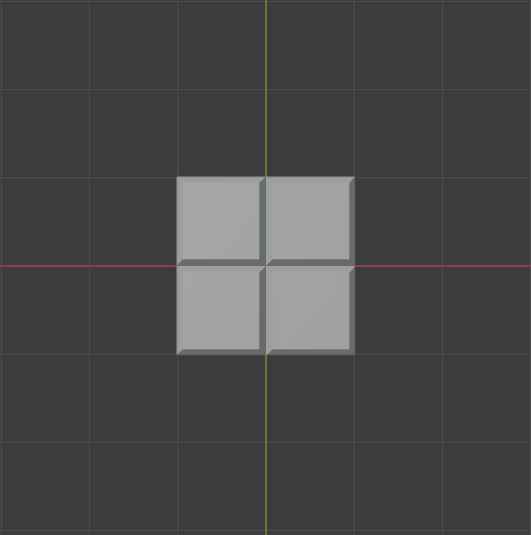
\includegraphics[width=50px]{../images/o.png}} 
  \subfigure[I]{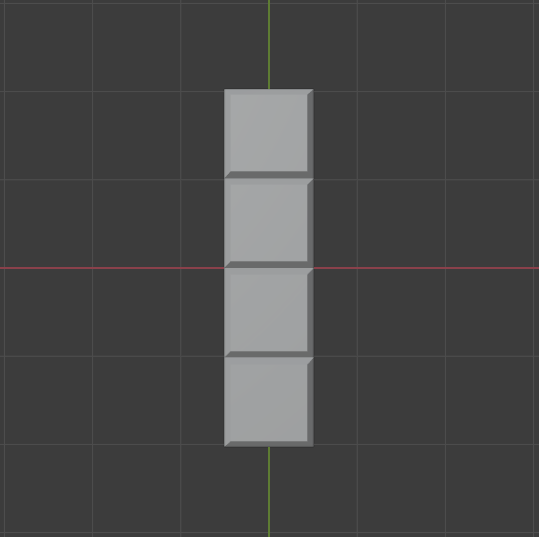
\includegraphics[width=50px]{../images/i.png}}
  \subfigure[S]{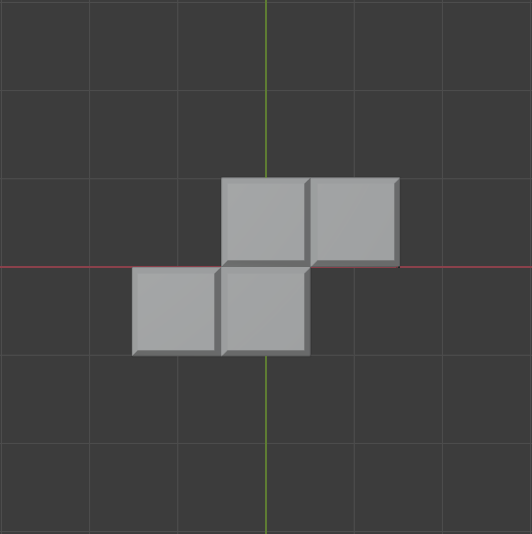
\includegraphics[width=50px]{../images/s.png}}
  \subfigure[Z]{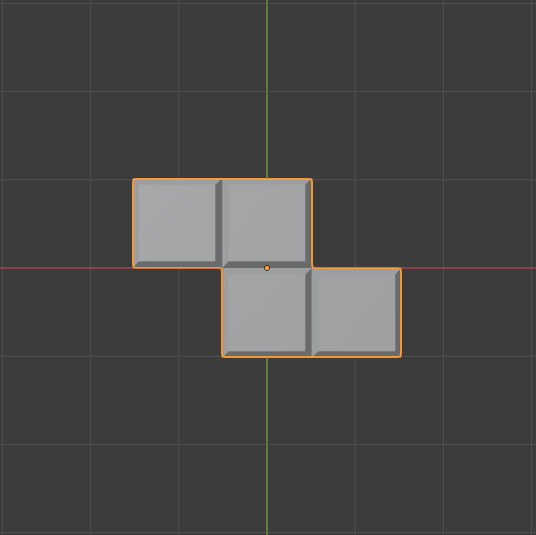
\includegraphics[width=50px]{../images/z.png}}
  \subfigure[J]{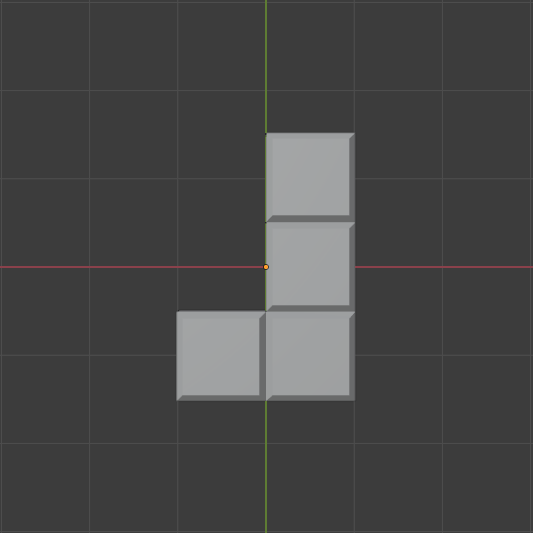
\includegraphics[width=50px]{../images/j.png}}
  \subfigure[L]{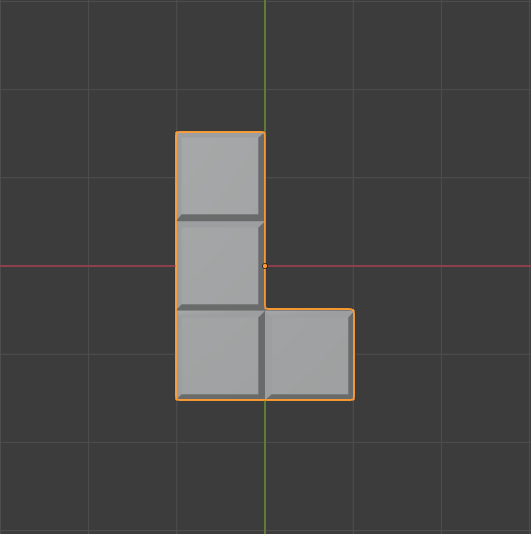
\includegraphics[width=50px]{../images/l.png}}
  \subfigure[T]{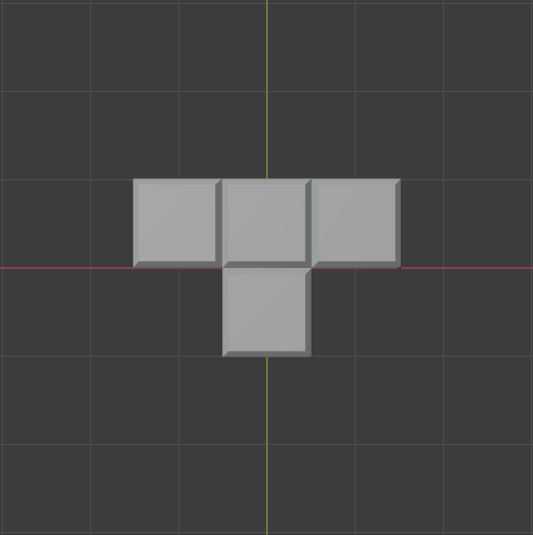
\includegraphics[width=50px]{../images/t.png}}
  \caption{\glspl{tet}}
  \label{tet-abb}
\end{figure}

\begin{wrapfigure}{r}{120px}
  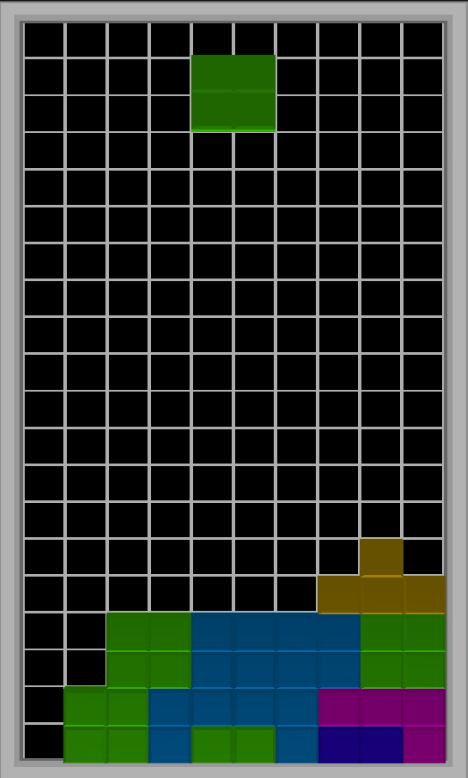
\includegraphics[width=120px]{../images/arena.png}
  \vspace{-20pt}
  \caption{Spielfeld (Arena)}
  \label{arena}
\end{wrapfigure}

Jedes mal wenn mindestens eine Zeile voll ist, wird diese entfernt und man erhält Punkte.
Je mehr Zeilen man gleichzeit füllt, umso mehr Punkte erhält. Jedoch kann man maximal 4 auf einmal voll sein, weil das längste \gls{tet} 
nur die Länge 4 hat (siehe \refabb{tet-abb}). Jedes mal, wenn 10 Zeilen entfernt wurden, erhöht sich das Level um 1.\cite{TetrisWiki}

Der Spieler kontrolliert ein herunterfallendes Tetromino, welches er allerdings nur nach links oder rechts bewegen kann.
Nach unten fällt es automatisch. Man kann den Fall beschleunigen aber nicht anhalten. 
Der Fall ist diskret, d.h. das aktuelle \gls{tet} immer nur nach einer bestimmten Zeit einen Block nach unten fällt.
Diese Zeit hängt vom Level ab und wird immer kürzer, umso höher es ist. Eine Begrenzung des Levels und somit der Fallgeschwindigkeit gibt es dabei nicht,
aber irgendwann ist es für Menschen nicht mehr machbar.
Die Objekte können auch rotiert werden, allerdings nur um 90 Grad Schritten. Somit haben die manche \glspl{tet} 4 Positionen, das O nur eine und I, S, Z nur 2.

Die \glspl{tet} dürfen während sie bewegt werden, nicht mit anderen Objekten in dem Spielfeld kolliederen und sich auch nicht aus dem Grenzen bewegen.
Wenn es eine Kollsion, nachdem das spielerkontrollierte Objekt gefallen ist, gibt, dann wird es in das Spielfeld platziert und fixiert. Es wird ein neues \gls{tet} 
zufällig generiert, welches am oberen Rand des Spielfelds startet.

Das Spiel endet, wenn ein Turm entstanden ist, der bis oben das Spielfeld füllt, sodass ein neues \gls{tet} sofort mit der Arena kollidiert.
Nachdem man das Spiel verloren hat, muss man von vorn beginnen, das Level und die Punkte werden zurück auf 0 gesetzt.

\subsection{Räumliche Transformationen}
% räumliche Projektion, Rotation, Skalierung
% Matritzen

\subsection{HSV - Farbraum}
% HSV - Farbraum

% Farbraum
Farbräume sind Modelle, mit denen man Farben durch Attribute definieren. 
Beispielsweise kann man eine Farbe durch ihren Grün-, Rot- und Blauanteil beschreiben oder 
durch die Sättigung, Helligkeit und Farbigkeit. Man kann solche Räume auch darstellen, indem man 
die Attribute als Koordinaten auffasst und dann z.B. in einem 3 dimensionalen Koordinatensystem abbildet. 
\cite{CS1}

% HSV Farbraum
In diesem Projekt kommt der HSV Farbraum zum Einsatz, welcher Helligkeit(V), Sättigung(S) und Farbigkeit(H).
Die ersten beiden werden linear interpretiert und die Farbigkeit ist ein Winkel auf dem, der per Definition auf eine Farbe abgebildet wird.
Die untere Abbildung verdeulicht diesen Zusammenhang noch einmal. 
\cite{CS2}
\begin{figure}[h]
  \centering
  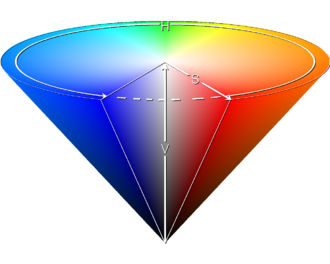
\includegraphics[width=200px]{../images/hsv.png}
  \caption{Darstellung HSV-Farbraum als Kegel}
\end{figure}

\pagebreak

\section{Codedokumentation}

% Sprache (C, GLSL)
% Bibliotheken (OPENGL, SDL2, bitmap, obj)

\subsection{Implementierung} 

\subsubsection{Gameengine} \label{gem}

Das Herz des Programms ist die \gls{geg}, welche die Logik der Objekte im Spiel kontrolliert.
Sie überprüft, ob Kollisionen stattfinden und berechnet z.B. die Punkte. 
Außerdem sorgt unsere Implementierung für das Speichermanagment der Spielobjekte.
Ihr gesamter Code befindet sich in \lstin{engine.c}.

Alle wichtigen Informationen werden zentral im \lstin{struct GameData} gespeichert.

Als erstes wird der Gamestate gespeichert, welcher den aktuellen Zustand des Spiels repräsentiert.
Er ist als \lstin{enum GameState} definiert, welcher 3 Einträge hat. 
\lstin{PLAYING} beschreibt den Hauptzustand, in dem der Spieler das fallende \gls{tet} bewegen kann und die Hintergrundmusik läuft.
Der Gamestate \lstin{PAUSE} kann durch den Spieler durch Drücken der P Taste erreicht werden. 
Darin werden alle Eingaben, die das aktuelle \gls{tet} bewegen ignoriert und die Hintergrundmusik ist stumm geschalten. Außerdem fällt kein Objekt.
Man kann durch erneutes Drücken von P das Spiel wieder in den Zustand \lstin{PLAYING} versetzen. Das Spiel geht dort weiter, wo es pausiert wurde.
\lstin{GAME_OVER} wird dann erreicht, wenn das Spiel verloren wurde (siehe \ref{def-tet}). 
Nun wird nur noch eine Nachricht angezeigt, dass der Spieler verloren und wie viele Punkte er erzielen konnte. Man kann das Spiel nun mit ESC beenden oder mit R neustarten.
Bei einem Neustart wird wieder in den \lstin{PLAYING}-Zustand übergagangen. Alle Zustandsinformationen werden resettet.

\begin{lstlisting}[language=C]
enum GameState {
    PAUSE,
    PLAYING,
    GAME_OVER
};

enum GameState gameState;
\end{lstlisting}

\refabb{state} zeigt eine Darstellung des Zustandsautomaten.

\begin{figure}[h]
  \centering
  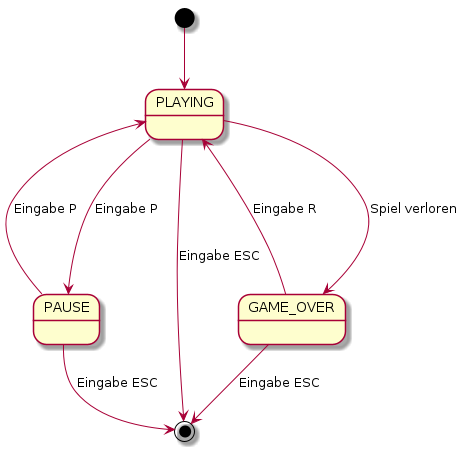
\includegraphics[width=0.5\textwidth]{../state.png}
  \caption{Zustandsautomat}
  \label{state}
\end{figure}

Die \glspl{tet} selbst sind als Matritzen definiert, die mithilfe vom eindimensionale Arrays dargestellt werden. Dabei stellt die 0 kein Block dar und 1-7 einen ausgefüllten Block.
Diese Zahl ist bei jedem Block unterschiedlich, weil durch sie später die Farbe des \gls{tet} bestimmt wird. Sie wird dann als Winkel für die Farbe im HSV-Farbraum verwendet.

Um dem Block an der Stelle $(x, y)$ zu erhalten, muss man diesen 2-dimensionalen Index eindeutig in einen 1-dimensionalen Arrayindex umwandeln. Dafür wurde folgende Formel verwendet:

\begin{figure}[h]
  \centering
  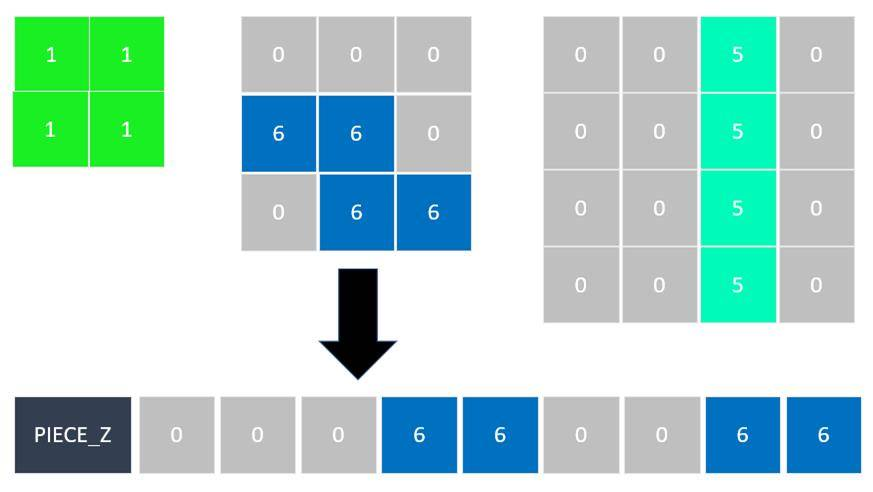
\includegraphics[width=200px]{../images/mem_layout.jpg}
  \caption{Speicherlayout \gls{tet}}
\end{figure}

\begin{center}
  \begin{math}
    i_{array} = x + y \cdot w
  \end{math}
\end{center}

Wobei $w$ die Breite der Matrix ist. (Die selbe Formel kann auch später für die Arena verwendet werden.)
Dafür muss man allerdings die Breite auch kennen. Deswegen wird am Anfang jeder Tetrominomatrix die Art gespeichert. Diese wird ebenfalls durch \lstin{enum} dargestellt.

\begin{lstlisting}[language=C]
enum Piece { PIECE_O, PIECE_L, PIECE_J, PIECE_T, PIECE_I, PIECE_Z, PIECE_S };
\end{lstlisting}

\lstin{arena} ist ein Pointer auf ein Array, dass die aktuelle Arena (Spielfeld) speichert. Sie ist 200 ($20 \cdot 10$) Elemente groß.
\begin{lstlisting}[language=C]
int* arena;  
\end{lstlisting}

Weil das Transformieren zwischen 2D und 1D Indizes werden muss, wurde dafür Helferfunktionen definiert. Außerdem wurde noch eine Macro definiert, die direkt Indices für die Arena ausrechnen kann, ohne ihre Breit explizit anzugeben.

\begin{lstlisting}[language=C]
#define COORDS_TO_ARENA_INDEX(x, y) (coords_to_array_index((x), (y), ARENA_WIDTH))

size_t coords_to_array_index(size_t x, size_t y, size_t width)
{ return y * width + x; }
\end{lstlisting}

\begin{wrapfigure}{l}{0px}
  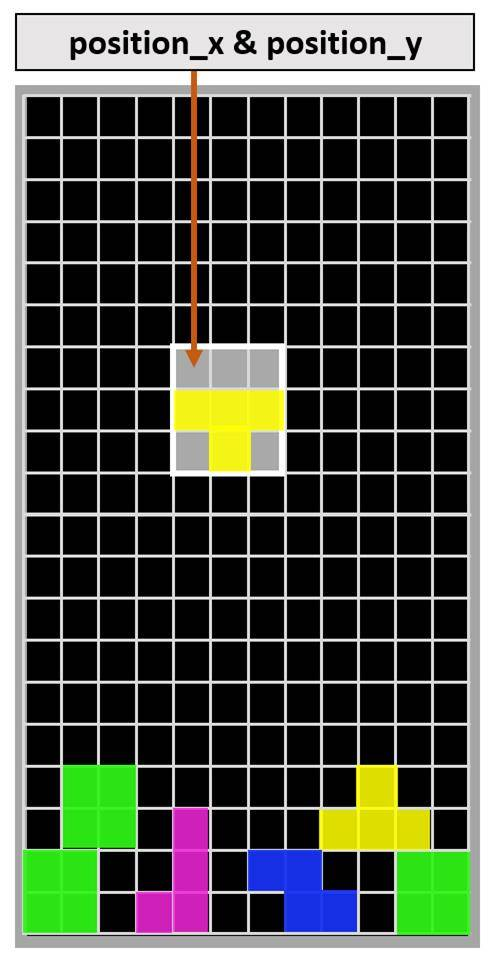
\includegraphics[width=120px]{../images/position.jpg}
  \vspace{-20pt}
  \caption{Position in der Arena}
  \vspace{-70pt}
\end{wrapfigure}

Diese beiden Integer speichern die aktuelle Arenaposition des \gls{tet}, dass durch den Nutzer kontrolliert wird.
\begin{lstlisting}[language=C]
int position_x;
int position_y;
\end{lstlisting}

Das folgenede Listing zeigt wichtige Metadaten über das Spiel. \lstin{score} wird ausschließlich für das Nutzerinterface benötigt und speichert die Punkte, die der Spieler erzielt.
Das \lstin{level} wird dem Spieler auch angezeigt, jedoch auch zur Berechnung der "Geschwingkeit" verwendet. 
Zusätzlich wird noch die Anzahl der gefüllten Zeilen in \lstin{cleared_lines} gespeichert, was dann zur Berechnung des aktuellen Levels genutzt wird.
Und \lstin{piece_count} ist ein Pointer auf ein Array, welches speichert, wie oft jedes Tetromino vorgekommen ist. Das wird rein visuell für das Nutzerinterface genutzt.

\begin{lstlisting}[language=C]
uint32_t score;
uint32_t level;
uint32_t cleared_lines;
int* piece_count;
\end{lstlisting}

Die Flag \lstin{bool fast_drop} speichert, ob der Spieler gerade den Knopf gedrückt hält, damit die Fallgeschwindigkeit seht stark erhöht wird.
Und \lstin{bool is_defeat} ist eine Flag, die im letzten Update im Zustand \lstin{PLAYING} gesetzt wird, um anzuzeigen, dass der Spieler verloren hat und der Gamestate auf \lstin{GAME_OVER} gesetzt wird.

Es wird auch der \lstin{seed}, der zum initialisieren des Zufallsgenerators genutzt wurde, gespeichert. Diese wird allerdings nicht weiter im Program verwendet (siehe \ref{uif}).
Das gleiche gilt für \lstin{accumulated_time};

Nun gibt es eine Reihe an Funktionen, die es erlauben, das aktuelle \gls{tet} bzw. dessen zu manipulieren und überprüfen, dass es nicht in einen unerlaubten Zustand kommt.

Dazu gehören als ersten die Funktionen, die nach Kollisionen mit den Wänden bzw. der Arena überprüfen. 
Das wurde mit 2 Helferfunktionen implementiert, die jeweils einer der beiden Fälle übernehmen.
Die Funktion \lstin{check_collision_arena_wall} evaluiert, ob der Spieler das aktuelle Objekt versucht aus der Arena herauszubewegen. 
Dafür muss aufgrund der Darstellung als Array, die erste Spalte von links bzw. rechts gefunden, nicht nur nullen enthält.
Dann wird zu \lstin{postion_x} der Index dieser Spalte hinzuaddiert und man erhält \lstin{non_zero_index_left}. Diese Zahl muss nun größer-gleich null sein, weil ansonsten die Begrenzung der Arena überschritten wurde.
Das gleiche gilt für rechts, nur das dort überprüft wird, das \lstin{position_x} addiert mit der ersten Spalte mit einem Enitrag, der nicht null ist, kleiner als die Breite der Arena ist.
Das untere Listing zeigt den Algorithmus beispielhaft für die Implementierung für die Kollisionabfrage mit der linken Wand. Für rechts ist so analog.
\begin{lstlisting}[language=C]
int size = get_piece_size(game_data->current_piece);
int non_zero_index_left = 0;
for (int x = 0; x < size; x++) {
    for (int y = 0; y < size; y++) {
        if (game_data->current_piece[coords_to_array_index(x, y, size) + 1] != 0) {
            non_zero_index_left = x;
            goto LOOP_END1;
        }
    }
}
LOOP_END1:;

return non_zero_left_index < 0; 
\end{lstlisting}

Die Funktion gibt allerdings \lstin{true} aus, wenn es eine Kollision gab, deswegen wird auf kleiner als null überprüft.

Desweitern gibt es \lstin{check_collision_arena_pieces}. Darin wird überprüft, ob das \lstin{current_piece} mit irgendeinem Objekt in der Arena kollidiert oder aus der Arena herausfällt.
Hier wird einfach über alle Einträge \lstin{current_piece} iteriert und geschaut, ob sich an der Position, wo in \lstin{current_piece} keine Null steht auch in der Arena keine null ist. 
Dann würde es zu einer Kollision kommen. Außerdem wird getestet, dass alle Einträge in aktuellen \gls{tet}, die eine $y$-Koordinate haben, die größer als die Höhe der Arena ist, null sind.
Ansonsten würde es aus der Arena fallen.

\begin{figure}[h]
  \centering
  \subfigure[Keine Wandkollision]{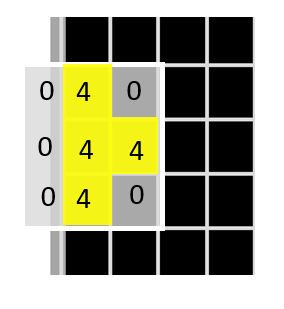
\includegraphics[height=100px]{../images/collision_wall_succ.png}}
  \hspace{40px}
  \subfigure[Wandkollision]{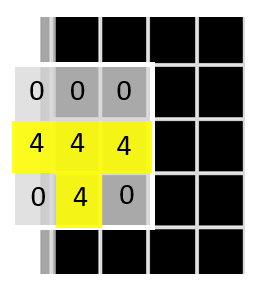
\includegraphics[height=100px]{../images/collision_wall_fail.png}}
  \hspace{40px}
  \subfigure[Kollision in der Arena]{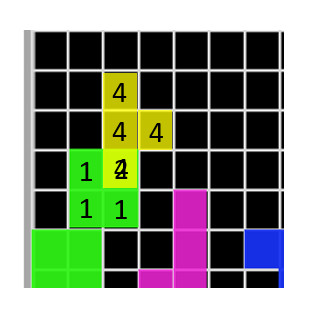
\includegraphics[height=105px]{../images/collision_pieces.png}}
  \caption{Kollisionsfälle}
\end{figure}

Die oben beschriebenen Helferfunktionen werden nun benötigt, wenn Objekte in der Arena bewegt werden sollen.
Dabei gibt es die horizontale Bewegung, die nur durch den Nutzer durchgeführt werden kann und das Fallen, 
das automatisch durch die Gameengine passiert.

Für die Bewegung durch den Nutzer ist die Funktion \lstin{move} zuständig. 
Die Funktion akzeptiert einen Pointer auf das aktuelle \lstin{struct GameData} Objekt und die Richtung, in die das aktuelle \gls{tet} bewegt werden soll.
Dann wird die Bewegung durchgeführt, und falls eine Kollision erkannt wird, wieder rückgängig gemacht. 
Diese Funktion wird dann durch den Eventhandler aufgerufen.
\begin{lstlisting}
void move(struct GameData* game_data, enum Direction dir)
{
    game_data->position_x += (dir == LEFT) ? -1 : 1;
    if (check_collision_side(game_data)) game_data->position_x -= (dir == LEFT) ? -1 : 1;
}  
\end{lstlisting}

Die Funktion, die das Fallen implementiert, heißt \lstin{drop}.
Sie übernimmt nicht nur die Bewegung, sondern muss auch, falls eine Kollision passiert, das aktuelle \gls{tet}
in die Arena schreiben, überprüfen, ob Zeilen gefüllt sind, die Punkte berechnen und dann gegebenenfalls ein neues \gls{tet} erstellen.

Grundsätzlich wird nur die $y$-Koordinate um eins erhöht und dann für eine Kollision geprüft.
Falls es eine gab, dann wird die $y$-Koordinate wieder dekrementiert und dann die oben beschriebenen Prozeduren durchgeführt, die alle als eigene Funktionen implementiert sind. 

\begin{lstlisting}
size_t drop(struct GameData* game_data)
{
    game_data->position_y++;
    size_t rows = 0;

    if (check_collision_arena_pieces(game_data)) {
        game_data->position_y--;

        write_piece_to_arena(game_data);
        rows = check_filled_rows(game_data);
        game_data->cleared_lines += rows;
        spawn_new_piece(game_data);
        level_up(game_data);
    }

    return rows;
}
\end{lstlisting}
\vspace{10pt}

\begin{wrapfigure}{r}{0px}
  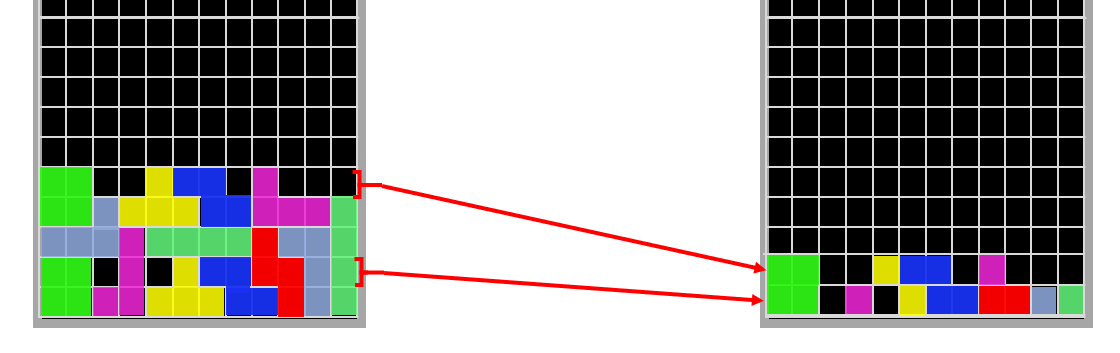
\includegraphics[width=220px]{../images/arena_copy.png}
  \caption{Schematische Darstellung: Entfernen von vollen Zeilen}
\end{wrapfigure}

\lstin{write_piece_to_arena}, \lstin{spawn_new_piece} und \lstin{level_up} sind in ihrer Implementierung trivial und werden deswegen hier nicht genauer beschrieben.


Interessanter ist hier die Funktion \lstin{check_filled_rows}, welche überprüft, ob es in der Arena volle Zeilen gibt, diese entfernt und dann die Punktzahl berechnet, welche der Spieler erhält. 

Sie iteriert von unten nach oben durch alle Zeilen der \lstin{arena} und speichert diese dann in \lstin{row_buffer} zwischen.
Danach werden die Punkte, die der Spieler erhält abhängig von der Anzahl der vollen Zeilen und dem aktuellen Level berechnet und direkt die Punktzahl in \lstin{game_data} erhöht.

Danach wird eine neue Arena generiert, in die die Zeilen aus der alten Arena kopiert werden. 
Dabei werden die Indizes beim Kopieren überprungen, die im \lstin{row_buffer}. Das hat den Effekt, 
dass die vollen entfernt Zeilen werden und allen anderen Zeilen entsprechend nach unten bewegt werden.
Am Ende wird der Pointer auf die Arena im \lstin{game_data} auf diese neue Arena gesetzt und der alte Speicher wird freigegeben.

\vspace{10pt}
\begin{lstlisting}
int* new_arena = (int*)calloc(sizeof(int), ARENA_WIDTH * ARENA_HEIGHT);
size_t current_row_index = ARENA_HEIGHT - 1;
buffer_index = 0;
for (int row = ARENA_HEIGHT - 1; row >= 0; row--) {
    if (row == row_buffer[buffer_index]) {
        buffer_index++;
        continue;
    }

    memcpy(new_arena + ARENA_WIDTH * current_row_index, game_data->arena + ARENA_WIDTH * row, sizeof(int) * ARENA_WIDTH);
    current_row_index--;
}

free(game_data->arena);
game_data->arena = new_arena;
\end{lstlisting}

Und die letzte wichtige Aufgabe der Gameengine ist das Rotieren der \glspl{tet}. Das wurde durch simple Matrixoperationen implementiert.
Um eine Matrix nach rechts zu rotieren, kann man sie transponieren und dann alle Zeilen umkeheren.
Und um dann eine Linksrotation durchzuführen kann man auch stattdessen 3 Rechtsrotationen ausführen.


\begin{figure}[h]
  
\begin{center}
  
$\begin{bmatrix}
  1 & 2 & 3\\
  4 & 5 & 6\\
  7 & 8 & 9
\end{bmatrix}$
$\xRightarrow[]{\text{Transponieren}}$
$\begin{bmatrix}
  1 & 4 & 7\\
  2 & 5 & 8\\
  3 & 6 & 9
\end{bmatrix}$
$\xRightarrow[]{\text{Zeilen umkehren}}$
$\begin{bmatrix}
  7 & 4 & 1\\
  8 & 5 & 2\\
  9 & 6 & 3
\end{bmatrix}$
\end{center}

\begin{center}
  
  $\begin{bmatrix}
    1 & 2 & 3\\
    4 & 5 & 6\\
    7 & 8 & 9
  \end{bmatrix}$
  $\xRightarrow[]{\text{Rechtsrotation}}$
  $\begin{bmatrix}
    7 & 4 & 1\\
    8 & 5 & 2\\
    9 & 6 & 3
  \end{bmatrix}$
  $\xRightarrow[]{\text{Rechtsrotation}}$
  $\begin{bmatrix}
    9 & 8 & 7\\
    6 & 5 & 4\\
    3 & 2 & 1
  \end{bmatrix}$
  $\xRightarrow[]{\text{Rechtsrotation}}$
  $\begin{bmatrix}
    3 & 6 & 9\\
    2 & 5 & 8\\
    1 & 4 & 7
  \end{bmatrix}$
\end{center}

\caption{Beispiel: Matrixrotationen}

\end{figure}

Um die Rechtsrotation effizienter zu Implementieren, kann man das Transponieren und Zeilen umkehren in einem Schritt erledigen.

Transponieren $t: a_{i,j} \mapsto a_{j,i}$, Zeilen umkehren $r: a_{ij} \mapsto a_{n-i,j}$ und damit $r \circ t: a_{i,j} \mapsto a_{n-j,i}$ ($n$ ist die Breite der Matrix).
Die obere Formel für $r \circ t$ wurde dann so im Code verwendet.
Die rotierte Matrix wird dann in einen Buffer gespeichert, der dann am Ende mit der Eingabematrix aus.
\begin{lstlisting}
for (size_t j = 0; j < size; j++) {
  for (size_t i = 0; i < size; i++) {
      size_t from_index = coords_to_array_index(i, j, size) + 1;
      size_t to_index   = coords_to_array_index(size - 1 -j, i, size) + 1;
      buffer[to_index] = (*piece)[from_index];
  }
}
\end{lstlisting}

\subsubsection{Rendern}

Das Rendern des Spiels auf dem Bildschirm wurde mithilfe von OpenGL implementiert. Das Fenster wird durch GLFW erzeugt.

Grundsätzlich gibt es 2 verschiedene Arten von Objekten, die gerendert werden müssen. Einmal die 3-dimensionalen Models wie z.B. die Begrenzung der Arena oder die \glspl{tet}. 
Andererseits die 2-dimensionalen Grafiken und die Texte.

Für das Rendern der Texte und Bilder wurde ein Model erstellt, welches eine Ebene darstellt. Diese wird dann mithilfe von Shadern im Raum platziert und das Bild wird als Textur verwendet.
Die Position des Bildes wird dann als Uniform in den Shadern gegeben. Zusätzlich kann man auch noch die Größe des Bildes angeben.
Der Fragmentshader rendert dann einfach die Texture auf die Ebene.
Beim Shader für die Schrift kann man allerdings nur die Position angeben.

\begin{lstlisting}
  uniform vec3 pos;
  uniform vec2 scale;
\end{lstlisting}
  
Dann wurden Helferfunktionen definiert, welche die Shader binden und die Funktionsaufrufe von OpenGL durchführen.
Ihre Signaturen kann man im unteren Listing sehen.

\begin{lstlisting}
  void draw_image(const user_data_t* user_data, GLint texunit, GLfloat* pos, GLfloat* scale);
  void draw_string(const user_data_t* user_data, const char* string, double pos_x, double pos_y);
\end{lstlisting}

Auf die Funktion \lstin{draw_string} sollte dabei nochmal etwas genauer eingegangen werden.
Sie kann nur Zahlen rendern, weil alle anderen Schriften durch Texturen dargestellt wurden.
Das geht bei den Zahlen leider nicht, weil diese im Userinterface veränderlich sind, 
weil sich z.B. die Punktzahl oder die Anzahl der gefüllten Zeilen während des Spiels erhöhen.

Das Rendern von Texten wurde nun so implementiert, dass für jede Ziffer von null bis neun eine Textur erstellt wurde.
In der Funktion \lstin{draw_string} wird dann über die Ziffern der zu zeichnenden Zahl iteriert 
und es werden nebeneinander die Bilder der entsprechenden Ziffern gerendert. 
Das kommt dadurch Zustande, dass zur $x$-Koordinate der Startposition ein Zeichenabstand addiert wird.  
Dabei ist der Zeichenabstand und die Schriftgröße konstant.
Man muss nur die richtige Textur vor dem Aufruf von \lstin{glDrawArrays} auswählen.

\begin{figure}[h]
  \centering
  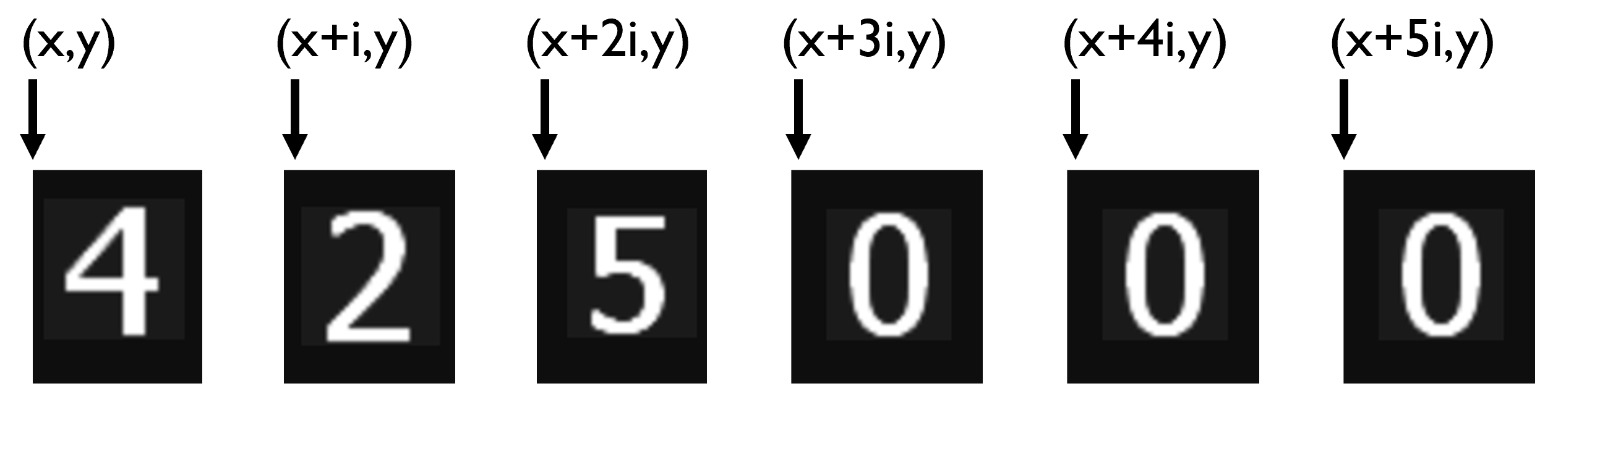
\includegraphics[width=400px]{../images/font.jpg}
  \caption{Rendern einer 6 stelligen Zahl (Schema)}
\end{figure}

\begin{lstlisting}
  double offset = 0.12;
  for (size_t i = 0; i < strlen(string); i++) {
      GLfloat pos[] = { pos_x + offset * i, pos_y };
      glUseProgram(user_data->shader_program_font);

      glUniform1i(user_data->digit_tex_uniform, (GLint)(string[i] - '0' + 1));
      glUniform2fv(user_data->digit_pos_uniform, 1, pos);

      glBindVertexArray(user_data->vao[2]);
      glBindBuffer(GL_ARRAY_BUFFER, user_data->vbo[2]);
      glDrawArrays(GL_TRIANGLES, 0, user_data->vertex_data_count[2]);
  }
\end{lstlisting}

Dann gibt es eine Reihe von Shadern, die die statischen Modelle rendern können.
Sie unterscheiden sich hauptächlich dadurch, 
dass die Position der verschiedenen Objekte in ihnen festgelegt ist. 
Objekte die auf diese Weise gezeichnet werden sind die Abgrenzung der Arena, die Modelle der \glspl{tet} im Userinterface.
Der Shader, der der die \glspl{tet} rendert, akzeptiert dabei wieder eine Position, weil sie sich in verschiedenen Positionen im Raum befinden.
Alle 3-dimensionalen Modelle werden perspektivisch dargestellt. Die räumliche Transformation von 3-d auf 2-d ist durch ein Frustum implementiert.
Außerdem wird danach noch ein Phong-Shading hinzugefügt.

Am komplizietersten werden die Tetrominos und die Arena selbst gerendert. 
Man hätte die Modelle einzeln in die Arena rendern können. 
Dieser Ansatz wäre jedoch sehr umständlich gewesen, weil man die enzelnen Modelle 
hätte rotieren müssen und teilweise hätte auseinander nehmen müssen, 
wenn sie teilweise durch das Entfernen der Zeilen auseinander genommen werden müssten.

Ein besserer Ansatz ist es, die Blöcke, aus denen die \glspl{tet} einzeln zu rendern.
Dafür wurde ein Modell für einen einzelnen Block erstellt. 
Da die Arena maximal 200 Blöcke enthalten kann, wurde sich in der Implementierung dafür entschieden, 
mithilfe von \lstin{glDrawArraysInstanced} nach jedem Update alle 200 Blöcke zu rendern. 
Im dafür zuständigen Vertexshader erhält man in der Variable \lstin{gl_InstanceID} 
den Index für den Block, der in diesem Aufruf des Shaders gerednet werden soll.

Somit kann man jetzt im Shader die Position von ihm berechnen:
\begin{lstlisting}
int x = gl_InstanceID % ARENA_WIDTH;
int y = gl_InstanceID / ARENA_WIDTH;
\end{lstlisting}
Das sind die $x$ und $y$-Koordinaten im Raster der Arena, die dann noch in Koordinaten im OpenGL Koordinatensystem umgerechnet werden.
Der Shader bekommt als \lstin{uniform} die gesamte Arena als Input.
So kann der Shader die Block-ID herausfinden, die er gerade rendert. Diese wird dann als Winkel für den HSV-Farbraum genommen, 
damit jedes Tetromino eine eigene Farbe bekommt.
Allerdings würde auf diese Weise das nutzerkontrollierte \gls{tet} nicht mit gezeichnet. 
Deswegen wurde noch eine Helferfunktion \lstin{generate_block_positions} definiert, welche die Arena und das nutzerkontrollierte \gls{tet} 
in einen Buffer kopiert und dieser wird dann dem Shader übergeben.

\begin{lstlisting}
uniform int block_positions[200];

block_id = block_positions[gl_InstanceID];
\end{lstlisting}

\begin{figure}
  $\begin{bmatrix}
    0 & 0 & 0 & 0 & 0\\
    0 & 0 & 0 & 0 & 0\\
    0 & 0 & 0 & 0 & 0\\
    0 & 0 & 0 & 0 & 0
  \end{bmatrix}$
  $\Rightarrow$
  $\begin{bmatrix}
    0 & 0 & 0 & 0 & 0\\
    0 & 0 & 0 & 0 & 0\\
    0 & 0 & 0 & 0 & 0\\
    0 & 0 & 0 & 0 & 0
  \end{bmatrix}$
  $\Rightarrow$
  
  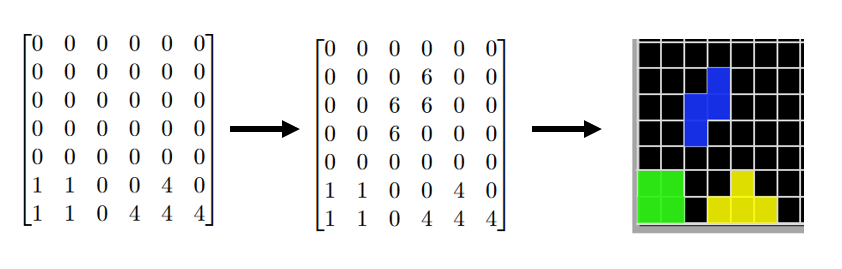
\includegraphics[width=200px]{../images/arena_halb.png}
  \caption{Renderprozess der Arena}
\end{figure}

Die Ausnahme stellt die Block-ID null dar. Sie ist ein Sentinel-Wert, der dem Fragment-Shader sagt, 
dass das aktuelle Fragment verworfen werden. Das wird dadurch realisiert, dass die ID vom Vertex zum Fragment Shader weitergegeben wird.
Der Fragmentshader überprüft dann, ob diese null ist und wenn ja wird \lstin{discard} aufgerufen.

Nun ist es so, dass auch die bestimmten Objekte abhängig vom Gamestate gezeigt werden oder nicht.
Wenn sich das Spiel im Zustand \lstin{PLAYING} oder \lstin{PAUSE} befindet, dann wird das gesamte Userinterface und die Arena mit den ganzen Blöcken gerendert.
Wenn sich das Programm allerdings im Zustand \lstin{GAME_OVER} ist, 
dann wird nur eine Textur mit der Nachricht, dass der Spieler verloren hat angezeigt und die erreichte Punktzahl. 

\subsubsection{Update}

Das Updaten und Rendern des Programm sind in der Implementierung 
auf Grund der Einfachheit der Logik und des Userinterfaces nicht getrennt. D.h. es gibt einen zentralen Mainloop, der zuerst die Funktion aufruft, 
die das gesamte Programm updated und anschließend rendert. Außerdem wird nach Events geprüft, die dann durch einen Eventhandler abgearbeitet werden.

Der Loop wird dann abgebrochen, wenn das Programm das Signal erhält, dass sich das Fenster schließen soll. 
Danach werden dann auch alle gelandenen Ressourcen (wie. z.B. Texturen, Musik, Modelle) wieder aus dem Speicher gelöscht.

\begin{lstlisting}
while (!glfwWindowShouldClose(window))
{
    update_gl(window);
    draw_gl(window);
    glfwSwapBuffers(window);
    glfwPollEvents();
}
\end{lstlisting}

\lstin{update_gl} selbst sorgt dafür, dass die Funktionen, die im Abschnitt \ref{gem} besprochen wurden, 
in der richtigen Reihenfolge und zur richtigen Zeit ausgeführt werden. Außerdem wird sich um das Managment der Gamestates und das Abspielen der Soundeffekte und der Hintergrundmusik gekümmert.

Das Timing wurde so implementiert, dass in jedem Update die aktuelle Zeit abgefragt wird. 
Die Zeit vom letzten Update wird zwischengespeichert. So kann man mit der aktuellen \lstin{frame_time} 
und der letzten die Zeit ausrechnen, die seit dem letzten Update vergangen ist.

\begin{lstlisting}
double frame_time = glfwGetTime();
double delta_time = frame_time - user_data->last_frame_time;
\end{lstlisting}

Diese \lstin{delta_time} kann man nun nutzen, um alle möglichen Funktionen in bestimmten Zeitintervallen auszuführen.

Das Fallen des \gls{tet} soll z.B. nur nach einer bestimmten Zeitspanne stattfinden, 
die sich mit steigendem Level erhöht, damit das Spiel schwerer wird. Das wurde so implementiert, 
dass \lstin{delta_time} in \lstin{time_since_last_drop} aufsummiert wird. Dann wird bei jedem Update überprüft, 
ob diese Summe größer ein bestimmtes Threshhold wird, dann wird \lstin{drop} ausgeführt. 
Dieses Threshhold ist nicht konstant, sondern eine Funktion vom aktuellen Level, die durch \lstin{calc_drop_time} berechnet wird.

\begin{wrapfigure}{r}{0pt}
  \centering
  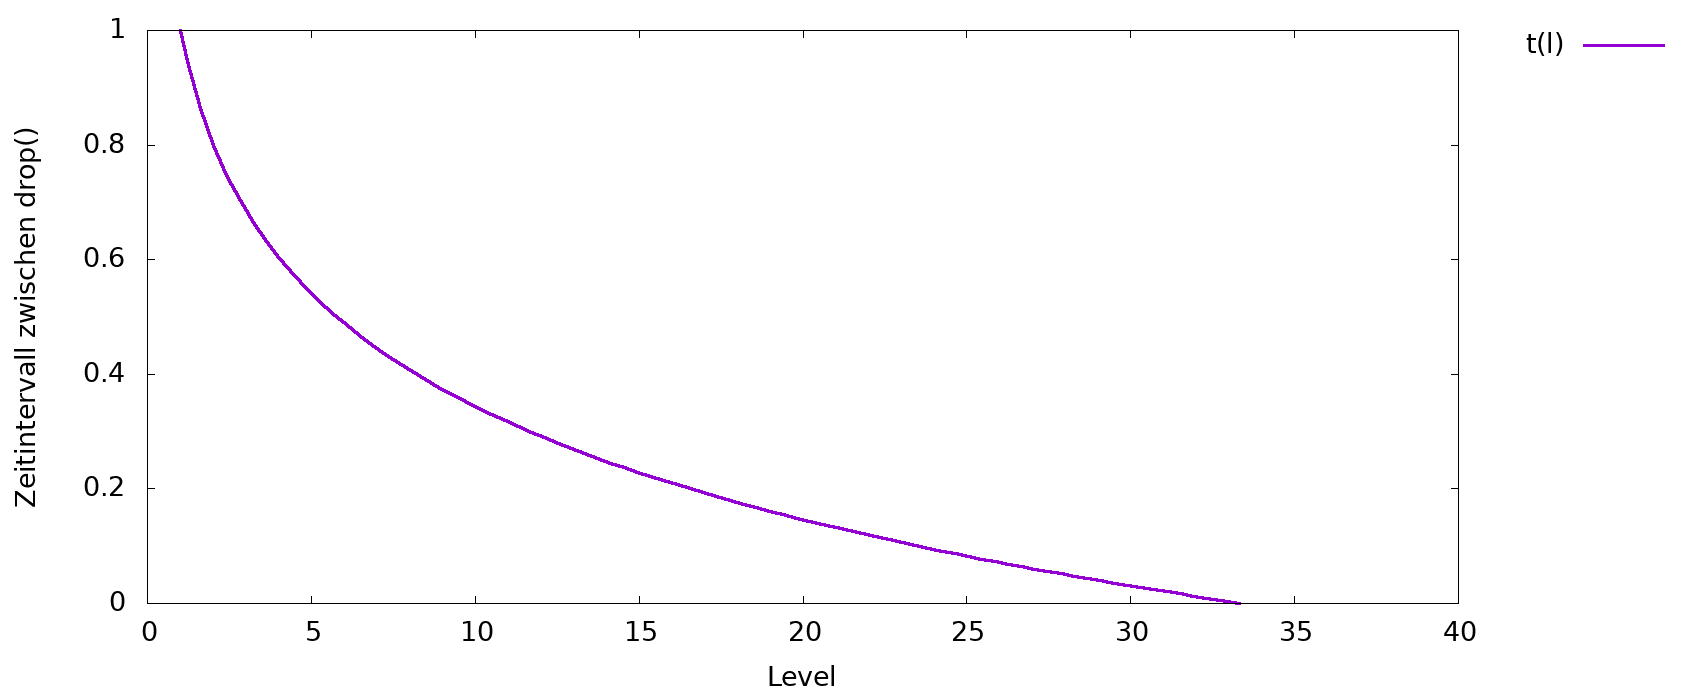
\includegraphics[width=200px]{../plt/level_speed.png}
  \caption{Level-Geschwingkeits-Funktion}
\end{wrapfigure}

\begin{center}
$t(l) = B - log(l + 1) * T$
\end{center}

$B$ und $T$ sind hier Konstanten, die durch probieren ermittelt wurden. Der Logarithmus wurde verwendet, 
damit die Zeit am Anfang schneller abfällt und sich dann immer langsamer der Nullstelle annähert. 
Das gibt den Leveln eine obere Begrenzung, weil die $t(33.2) \approx 0$, und das Spiel auch schon davor für einen menschlichen Spieler zu schnell wird.  
Der Nutzer kann allerdings durch Drücken von S das Zeitintervall sehr stark verkürzen, sodass das \gls{tet} sehr schnell wird.
Dafür wird die aufsummierte Zeit mit \lstin{FAST_DROP_TIME} abgeglichen, was eine sehr kleine Konstante ist.
Das wurde so realisiert, dass überprüft wird, ob die \lstin{fast_drop}-Flag \lstin{true} ist. Die ganze Bediengung kann im unteren Listing betrachtet werden.

\begin{lstlisting}
  (!user_data->gameData.fast_drop && (user_data->time_since_last_drop >= calc_drop_time(&user_data->gameData))) ||
  (user_data->gameData.fast_drop && user_data->time_since_last_drop >= FAST_DROP_TIME)
\end{lstlisting}

Wie man sehen kann, gibt \lstin{drop} die Anzahl der gefüllten Zeilen aus. Wenn es 4 sind, wird ein spezieller Soundeffekt abgespielt.
Danach wird die aufsummierte Zeit wieder auf null gesetzt, damit der ganze Update-Zyklus von neuem beginnen kann.
Am Ende wird noch überprüft, ob die \lstin{is_defeat}-Flag von der Gameengine gesetzt wurde, 
was signalisiert, dass der Spieler verloren hat. In diesem Fall wird der Gamestate auf \lstin{GAME_OVER} 
gesetzt und auch hier wird dann der entsprechende Soundeffekt abgespielt. 

\begin{lstlisting}
if (...) {
    size_t cleared_rows = drop(&user_data->gameData);

    if (cleared_rows == 4) queue_audio_if_empty(user_data->effect_device, user_data->wav_data[2]);
    user_data->time_since_last_drop = 0.0;

    if (user_data->gameData.is_defeat) {
        queue_audio_if_empty(user_data->effect_device, user_data->wav_data[1]);
        user_data->gameData.gameState = GAME_OVER;
    }
}
\end{lstlisting}

Zusätzlich wurde dem Nutzer die Möglichkeit gegeben, die Tasten zum Bewegen der \glspl{tet} gedrückt zu halten.
Dafür wurde ähnlich wie oben wieder eine Variable erstellt, die \lstin{delta_time} 
aufsummiert und überprüft, ob ein konstater Wert überschritten wurde. 
Dann kann mithilfe der Flags \lstin{holding_left} bzw. \lstin{holding_right} festgestellt werden, 
in welche Richtung sich bewegt werden soll. So wird die Bewegung innerhalb 
eines bestimmten Zeitintervalls periodisch ausgeführt und der Spieler musst die Tasten A und D nicht andauern drücken.

\begin{lstlisting}
  if (user_data->time_since_last_side_move >= MOVE_SIDE_WAYS_TIME) {
      enum Direction dir;
      if (user_data->holding_left)  dir = LEFT;
      if (user_data->holding_right) dir = RIGHT;
      move(&user_data->gameData, dir);
      user_data->time_since_last_side_move -= MOVE_SIDE_WAYS_TIME;
  }
\end{lstlisting}
  
Die beiden gerade beschriebenen Prozeduren werden nur ausgeführt, wenn sich das Programm um Zustand \lstin{PLAYING} befindet.
In den anderen beiden Zuständen finden keine Updates statt. Außerdem wird im Zustand \lstin{PAUSE} noch die Hintergrundmusik pausiert.

\begin{lstlisting}
  (user_data->gameData.gameState == PAUSE) ? pause(user_data->background_device) : unpause(user_data->background_device);
\end{lstlisting}

Zusätzlich gibt es noch einen Eventhandler, der die Eingabeevents von der Tastatur behandelt. Dieser wurde mithilfe von GLFW implementiert.
Grundsätzlich wird nur überprüft, welche Taste der Nutzer gedrückt hat und dann wird entsprechend nach Gamestate gehandelt.
Der Code ist so trivial, dass er hier nicht weiter besprochen wird.

\subsubsection{Audio}

Für das Abspielen der Hintergrundmusik und den Soundeffekten wurde die Bibliothek SDL2 verwendet.
Damit die Musik unabhängig von den Effekten ist, wurden zwei verschiedene \lstin{audio_devices} geöffnet, die man sich als Audiokanäle vorstellen kann. 

Man kann in diese Kanäle Audiodaten einreihen, weil sie wie eine Warteschlange funktioniert, die die Audiosamples nacheinander abspielt.

Die Musik und Soundeffekte sind in WAV-Datein gespeichert, die durch SDL geladen werden und deren Daten dann im \lstin{struct WavData} gespeichert werden.
\begin{lstlisting}
struct WavData {
    SDL_AudioSpec wav_spec;
    Uint32 wav_length;
    Uint8* wav_buffer;
};
\end{lstlisting}

Zum Einreihen in die Audiokanäle wurden 2 Helferfunktionen implementiert. \lstin{queue_audio} fügt die Samples einfach in die Warteschlange ein, ohne zu überprüfen, ob sie leer ist.
Und die Funktion \lstin{queue_audio_if_empty} überprüft erst, ob die Warteschlange bereits ist und ruft dann \lstin{queue_audio} auf.

Das Abspielen der Hintergrundmusik wurde dann so implementiert, dass einfach nach jedem Update \lstin{queue_audio_if_empty} aufgerufen wird, 
sodass die Musik wiederholt, falls das Lied vorbei ist.

Beim Abspielen von Soundeffekten wird ebenfalls diese Funktion aufgerufen, sodass Soundeffekte verworfen werden, falls sie gleichzeitig abgespielt werden sollen.

\subsection{Userinterface}
Das Userinterface ist sehr einfach gehalten. Alle Nutzereingaben erfolgen über die Tastatur. 
Das Tastaturlayout wird genauer im Kapitel \ref{geb} geschrieben.

Auf der linken Seite des Bildschirms wird eine Liste mit den \glspl{tet} angezeigt, die die absoluten Häufigkeiten angibt, 
wie oft man welche Form erhalten hat. 
Zentral im Fenster kann man die Arena sehen, die den Hauptinhalt des Spiels darstellt. Darunter befindet sich ein kleiner Schriftzug, der eine Beschreibung des Tastaturlayouts beschreibt.

Rechts wird dann untereinander angezeigt, welches \gls{tet} als nächstes vorkommt, die Punktzahl des Spieler, welches Level bis jetzt erreicht wurde und wieviele Zeilen bis jetzt gefüllt wurden.
Falls der Nutzer das Spiel verliert, wird mittig auf dem Bildschirm dann ein Text angezeigt, der dem Spieler anzeigt, dass das Spiel vorbei ist, seine Punktzahl und wie
er das Programm beenden kann oder eine neue Runde starten.

\subsection{Nicht implementierte Features} \label{uif}

Auffällig ist, dass es kein Hauptmenü gibt, sondern der Spieler sofort ins Spiel geworfen wird. 
In so einem Menü könnte man dann auch noch verschiedene Einstellungsmöglichkeiten unterbringen, z.B., 
dass man die Musik- und Effektlautstärtke anpassen kann, die Tastenbelegung ändern kann und das Farbschema anpassen kann.
Außerdem könnte man einen Menüpunkt "Bestenliste" implementieren, der dann die Highscores verschiedener Spieler in einem Extrafenster anzeigen lässt.
Dazu müsste auch ein Speichersystem erstellen, welches die Punktzahlen in einer lokalen Datei oder z.B. auf einem Webserver speichert.

Man kann auch im Code einige Stellen finden, in dem der \lstin{seed} des Zufallsgenerators gespeichert wird. Es war ursprünglich geplant, 
dass es die Möglichkeit gibt, diesen per Hand zu setzten. Das wurde jedoch auch noch nicht implementiert.

Und man könnte auch noch ein kleines Tutorial oder eine Spielanleitung einfügen, falls der Spieler nicht mit den Regeln von Tetris vertraut ist.

Für fortgeschrittene Spieler wäre aus denkbar, dass man das Startlevel benutzerdefiniertbar macht, sodass diese nicht immer bei Level null anfangen müssen,
sondern direkt in ein höheres Level einsteigen können.
\pagebreak

\section{Projektdokumentation}

\subsection{Tools \& Bibliotheken}

\textbf{Genutzte Tools:}
\begin{itemize}
  \item Versionskontrolle: Github \& git
  \item Codeeditor: VS Code
  \item Textverarbeitung: \LaTeX
  \item Zustandsdiagramme: plantUml
  \item Diagramme: gnuplot
  \item Abbildungen: Powerpoint
  \item 3-D Modellierung: Blender
  \item Compiler: gcc
  \item Debugger: gdb, valgrind
  \item Buildtools: make
  \item Bildverarbeitung: Krita
\end{itemize}

\noindent \textbf{Genutzte Programm-Bibliotheken:}
\begin{itemize}
  \item OpenGL
  \item SDL2
  \item glad
  \item GLFW
  \item Bitmap-Bibliothek
  \item Obj-Bibliothek
\end{itemize}

\subsection{Arbeitsaufteilung}

\section{Benutzerhandbuch}

\subsection{Installation}

\begin{lstlisting}[language=bash]
$ git clone 
$ cd MultimediaProjekt
$ make all
$ ./teris.out
\end{lstlisting}

Das Programm kann mit der Makefile momentan nur für Linux kompiliert werden. Getstet wurde es auf Ubuntu 20.04. 
Dafür muss OpenGL und GLFW installiert sein. SDL2 ist optional. Falls diese Bibliothek fehlt, 
dann wird ohne sie kompiliert und es gibt keine Musik und keine Soundeffekt.

Zudem braucht man eine Tastatur, um das Programm zu bedienen.

\subsection{Gebrauchsanleitung} \label{geb}
Zum Starten des Spiels klickt man zweimal schnell auf „Tetris.out“ und damit startet das Spiel automatisch.  
Es beginnt damit, dass nun die zufällig generierten „\glspl {tet}“ in die Arena reinfallen. Jetzt ist die Aufgabe des Spielenden, die „\glspl {tet}“ so zu platzieren, dass diese vollen Reihen möglichst ohne Lücken erzeugen. 


Es löhnt sich, mehr Zahlen auf einmal wegzuschaffen, denn die Punktzahl nicht linear mit der Anzahl von Reihen skaliert.  Z. B. beim Level null, wenn vier Reihen auf einmal weggemacht werden, kriegt der Spielende 1200 Punkte. Mach der Spielende vier Zahlen nacheinander, erreicht er nur 160 Punkte (40 Punkte je eine Reihe). 
Die Anzahl der Punkte, die erhalten wird, hängt auch vom Level ab (nach jeweils 10 gelöschten Zeilen erhöht sich das Level um eins und damit die Geschwindigkeit, mit der „\glspl {tet}“ fallen).

Das Spiel endet, sobald eine Figur nicht mehr auf das Spielfeld passt und ein Teil davon außerhalb des Spielfelds liegt. Die Punkte hören auf zu zählen, die Figuren bewegen sich nicht, und es erscheint ein Fenster, das dem Benutzer mitteilt, dass das Spiel beendet ist und er eine bestimmte Anzahl von Punkten erreicht hat.

\begin{figure}[h]
  \centering
  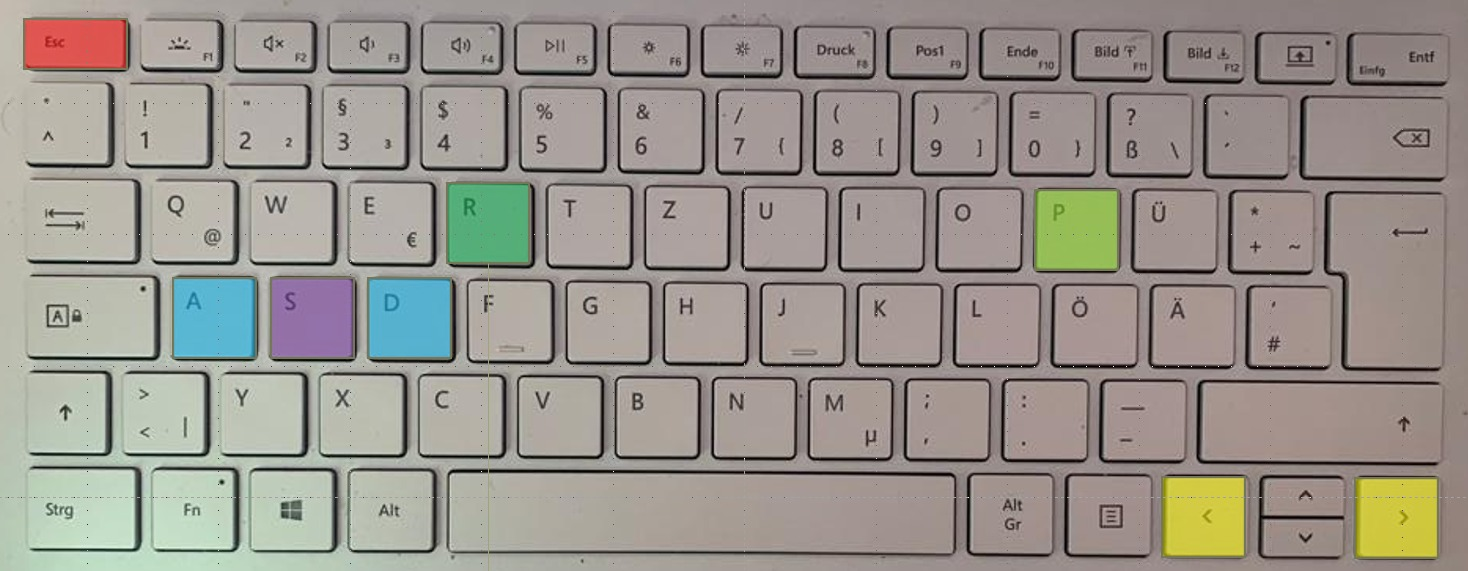
\includegraphics[width=400px]{../images/keyboard.jpg}
  \caption{Tastaturlayout}
  \label{tat}
\end{figure}

Um die „\glspl {tet}“ zu steuern, wurden die verschiedenen Befehle vorgesehen. Die Tasten, die dazu benutzt werden, sind in der Abbildung \ref{tat} dargestellt.


Die blauen markierten Tasten („A“ und „D“) werden verwendet, um „\glspl {tet}“ nach links und rechts zu bewegen. Wenn die Taste "A" ("D") lange gedrückt gehalten wird, bewegt sich das „\gls {tet}“ sofort an den linken (rechten) Rand des Spielfelds. Für die Rotation der „\glspl {tet}“ sind die Falltasten „links“ (Rotation nach links) und „rechts“ (Rotation nach rechts) bestimmt.  Um das Spiel zu pausieren, muss die Taste "P" gedrückt werden. Nachdem die Taste „P“ nochmal betätigt wird, setzt sich das Spiel fort. Zum Beenden des Spiels kann entweder die Taste „Esc“ oder der Kreutz genutzt werden.  Wenn man die Taste "R" drückt, wird das Spiel neu gestartet.  

Außerdem könnte die Größe vom Spielfenster angepasst werden.  


\pagebreak
\bibliographystyle{alpha}
\bibliography{references} % see references.bib for bibliography management

\end{document}

% for citation:
% \cite{aad} for simple citation
% \cite[S. 20]{aad} for citation with page number(s)

% for acronyms and glossary ref:
% https://en.wikibooks.org/wiki/LaTeX/Glossary
% \gls{acro-name}

% Listings Example:
% \begin{lstlisting}[language=C]
%         #include <stdio.h>
%        
%         int main(void)
%         {
%                 printf("Hello, World\n");
%                 return EXIT_SUCCESS;
%         }
% \end{lstlisting}

% TODO: 
% Definitions
% Reference for Stackoverflow recursion depth in defs and traversal
% Pictures for tree and for tree array represantation